\graphicspath{{./images/chap3/}}
% Relevance Feedback
% Methodology
% * Design and Architecture
% * Population of interest and sampling subject used in the study
% * Instrument and what it measures (matrices)
% * qualifications of informants if used in the study
% * Validation
% * Data gathering procedure (experiments)
\chapter{Datasets} % (fold)
\label{cha:datasets}

All the experiments in this study are conducted on a database which comprises two
species of skinks: \emph{Grand} and \emph{Otago} of 3687 images in total
created by biologists at New Zealand's Department of Conservation.

\begin{figure}[htb]
  \centering
  \begin{subfigure}[t]{0.31\textwidth}
      \centering
      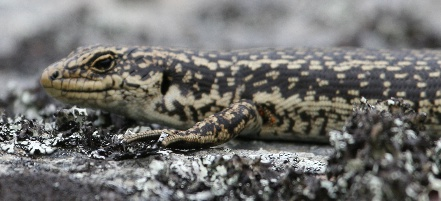
\includegraphics[width=4.5cm]{dataset/general/grand_L3}
  \end{subfigure}
  \begin{subfigure}[t]{0.31\textwidth}
      \centering
      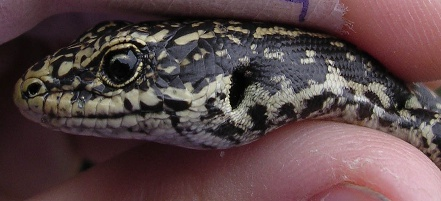
\includegraphics[width=4.5cm]{dataset/general/grand_L1}
  \end{subfigure}
  \begin{subfigure}[t]{0.31\textwidth}
      \centering
      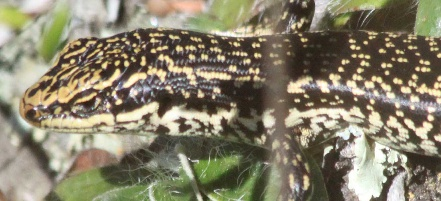
\includegraphics[width=4.5cm]{dataset/general/grand_L2}
  \end{subfigure}
  \captionsetup{justification=centering}
  \caption{Left view images from Grand dataset}
  \label{fig:grand_left} %chktex 24
\end{figure}

\begin{figure}[htb]
  \centering
  \begin{subfigure}[t]{0.31\textwidth}
      \centering
      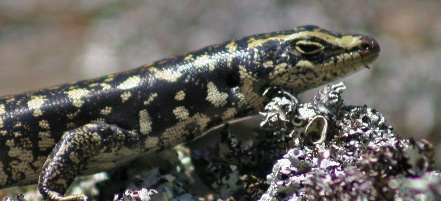
\includegraphics[width=4.5cm]{dataset/general/otago_R2}
  \end{subfigure}%
  \begin{subfigure}[t]{0.31\textwidth}
      \centering
      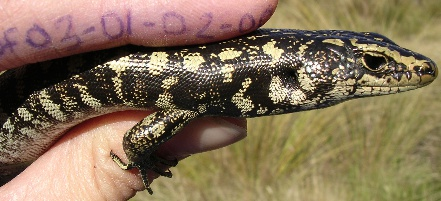
\includegraphics[width=4.5cm]{dataset/general/otago_R1}
  \end{subfigure}
  \begin{subfigure}[t]{0.31\textwidth}
      \centering
      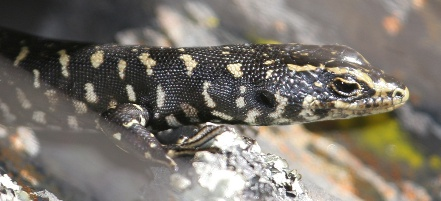
\includegraphics[width=4.5cm]{dataset/general/otago_R3}
  \end{subfigure}
  \captionsetup{justification=centering}
  \caption{Right view images from the Otago dataset}
  \label{fig:otago_right} %chktex 24
\end{figure}

The Grand database contains 1871 \texttt{RGB} images of 206 individuals, while
the Otago database contains 1816. These images vary in size, lighting, and
background. The images are closely cropped to include only the anterior end of
their subjects. The size varies from 1056 $\times$ 564 to 2437 $\times$ 1215
pixels.

\begin{table}[htb]
\captionsetup{justification=centering}
  \caption{Summary of each database}
  \label{tab:database_summary} %chktex 24
  \centering
  \begin{tabular}{lccccccc}
    \toprule
    & \multicolumn{3}{c}{Number of Images} & & &
        \multicolumn{2}{c}{Images per Individual} \\
    \cmidrule{2-4}
    \cmidrule{7-8}
    Name & Left View & Right View & Total & Individuals & Singletons & Avg.
        & Max. \\
    \midrule
    Grand & 929 & 942 & 1871 & 206  & 69 & 9 & 31 \\
    Otago & 903 & 913 & 1816 & 221  & 58 & 8 & 24 \\
    \bottomrule
  \end{tabular}
\end{table}


\section{General}

\subsection{Selfscore and Score Distributions}

Sloop ranks the likelihood that two capture events contain the same individuals
quantitatively by \emph{similarity score}. The similarity score between two
individuals is obtained from comparing the SIFT features of all the images
within a capture to the SIFT features of the images within the other
individual's cohort.  These scores are normalized by the \emph{minimum
selfscore} among all the images involved in the
comparison. A \emph{capture} is a group of images containing the same
individual from different views, captured at the same time.  A \emph{cohort} is
a set of all images from all captures of the same individual.

\subsubsection{Selfscores}

The selfscore for a capture is the \emph{maximum} selfscore of all the images within
the capture, where a selfscore of an image is calculated from comparing the
sift features of each image with itself.
$$\texttt{selfscore}(C) = \max_{\forall I_i \in C} \texttt{sift\_match}(I_i, I_i)$$

\begin{figure}[htb]
   \centering
    \begin{subfigure}[t]{0.6\textwidth}
        \centering
        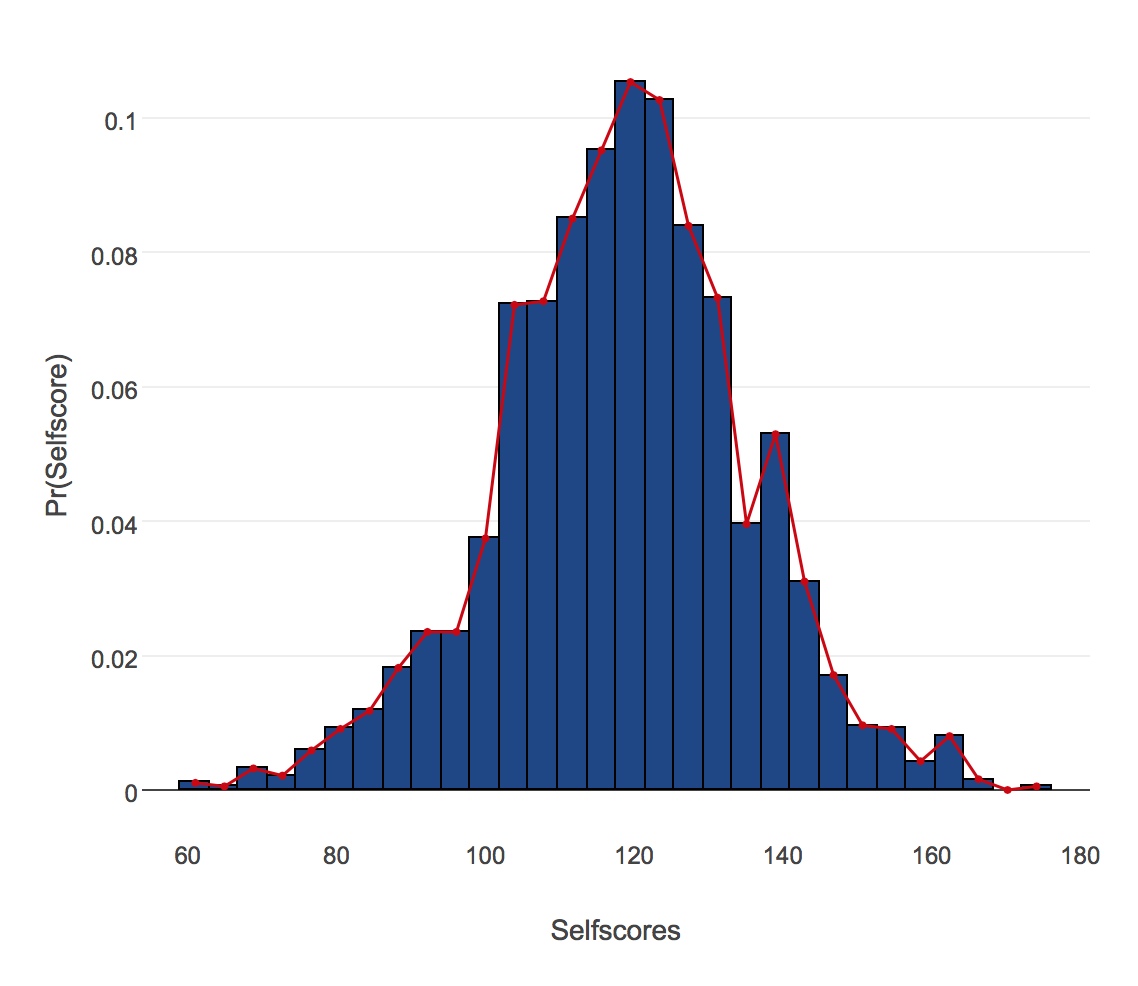
\includegraphics[height=2.5in]{dataset/grand/selfscores}
        \caption{Probability distribution}
    \end{subfigure}%
    \begin{subfigure}[t]{0.35\textwidth}
        \centering
        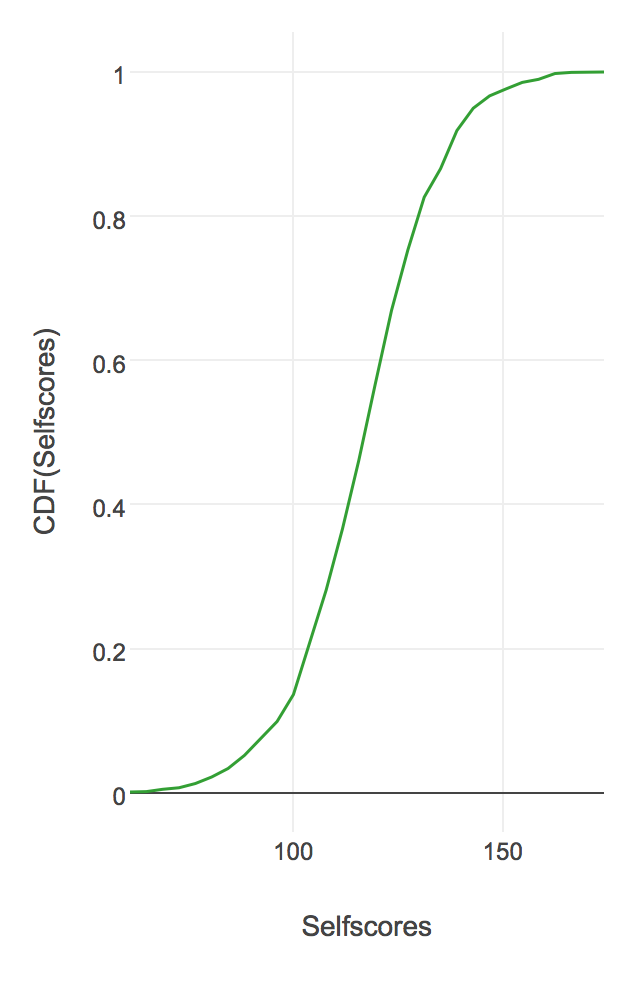
\includegraphics[height=2.5in]{dataset/grand/cdf_selfscores}
        \caption{Cumulative probability distribution}
    \end{subfigure}
    \caption{Grand selfscores}

    \begin{subfigure}[t]{0.6\textwidth}
        \centering
        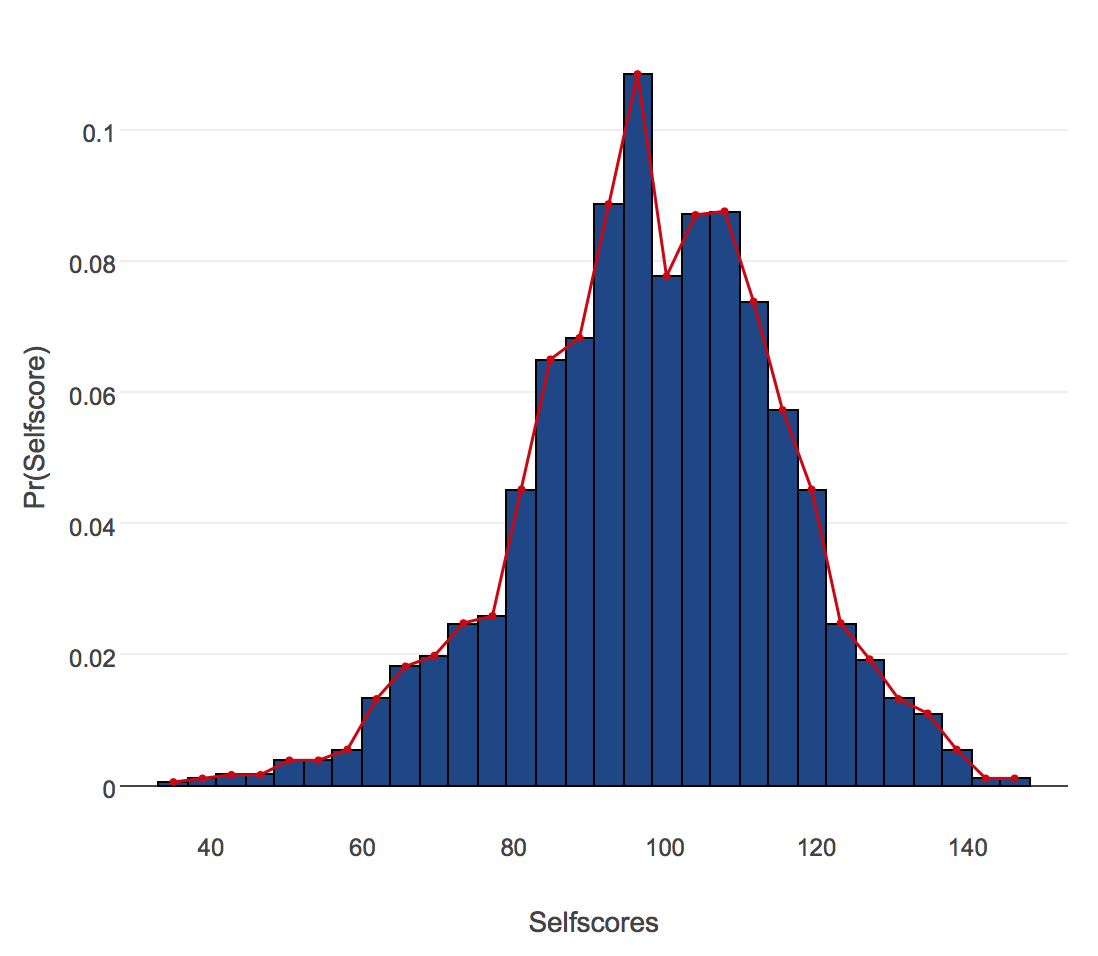
\includegraphics[height=2.5in]{dataset/otago/selfscores}
        \caption{Probability distribution}
    \end{subfigure}%
    \begin{subfigure}[t]{0.35\textwidth}
        \centering
        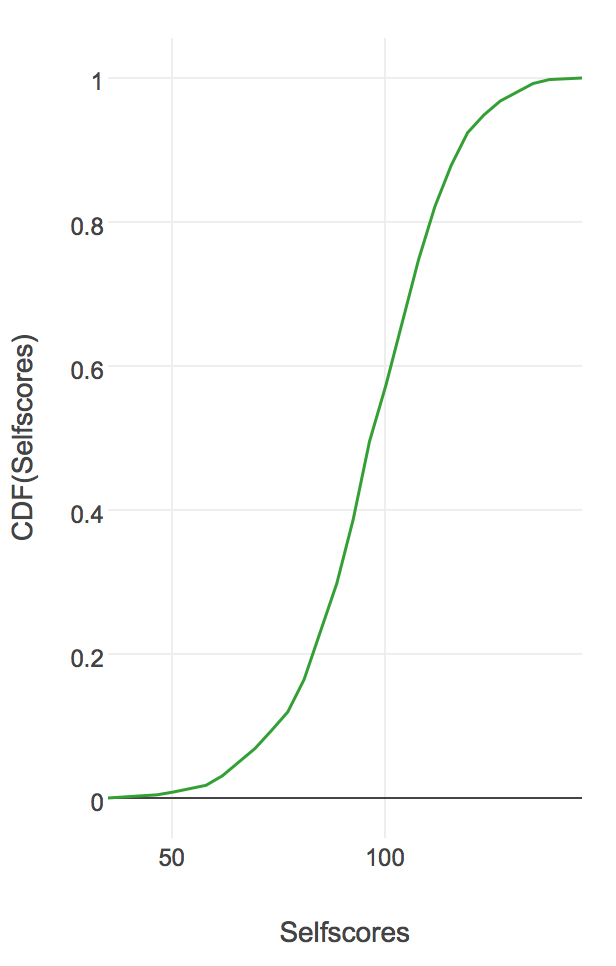
\includegraphics[height=2.5in]{dataset/otago/cdf_selfscores}
        \caption{Cumulative probability distribution}
    \end{subfigure}
    \caption{Otago selfscores}
\end{figure}

\subsubsection{Scores}

The score between the two individuals is the maximum score among all the
comparisons among the images within the two cohorts.
$$\texttt{score}(C_1, C_2) = \max_{\forall I_i \in C_1 \forall I_j \in C_2}
    \frac{\texttt{sift\_match}(I_i, I_j)}{\min(\texttt{selfscore}(C_1),
        \texttt{selfscore}(C_2))}$$
where $C$ is a capture and $I$ is an image in a capture.

\begin{figure}[htb]
 \begin{subfigure}[t]{\textwidth}
  \centering
  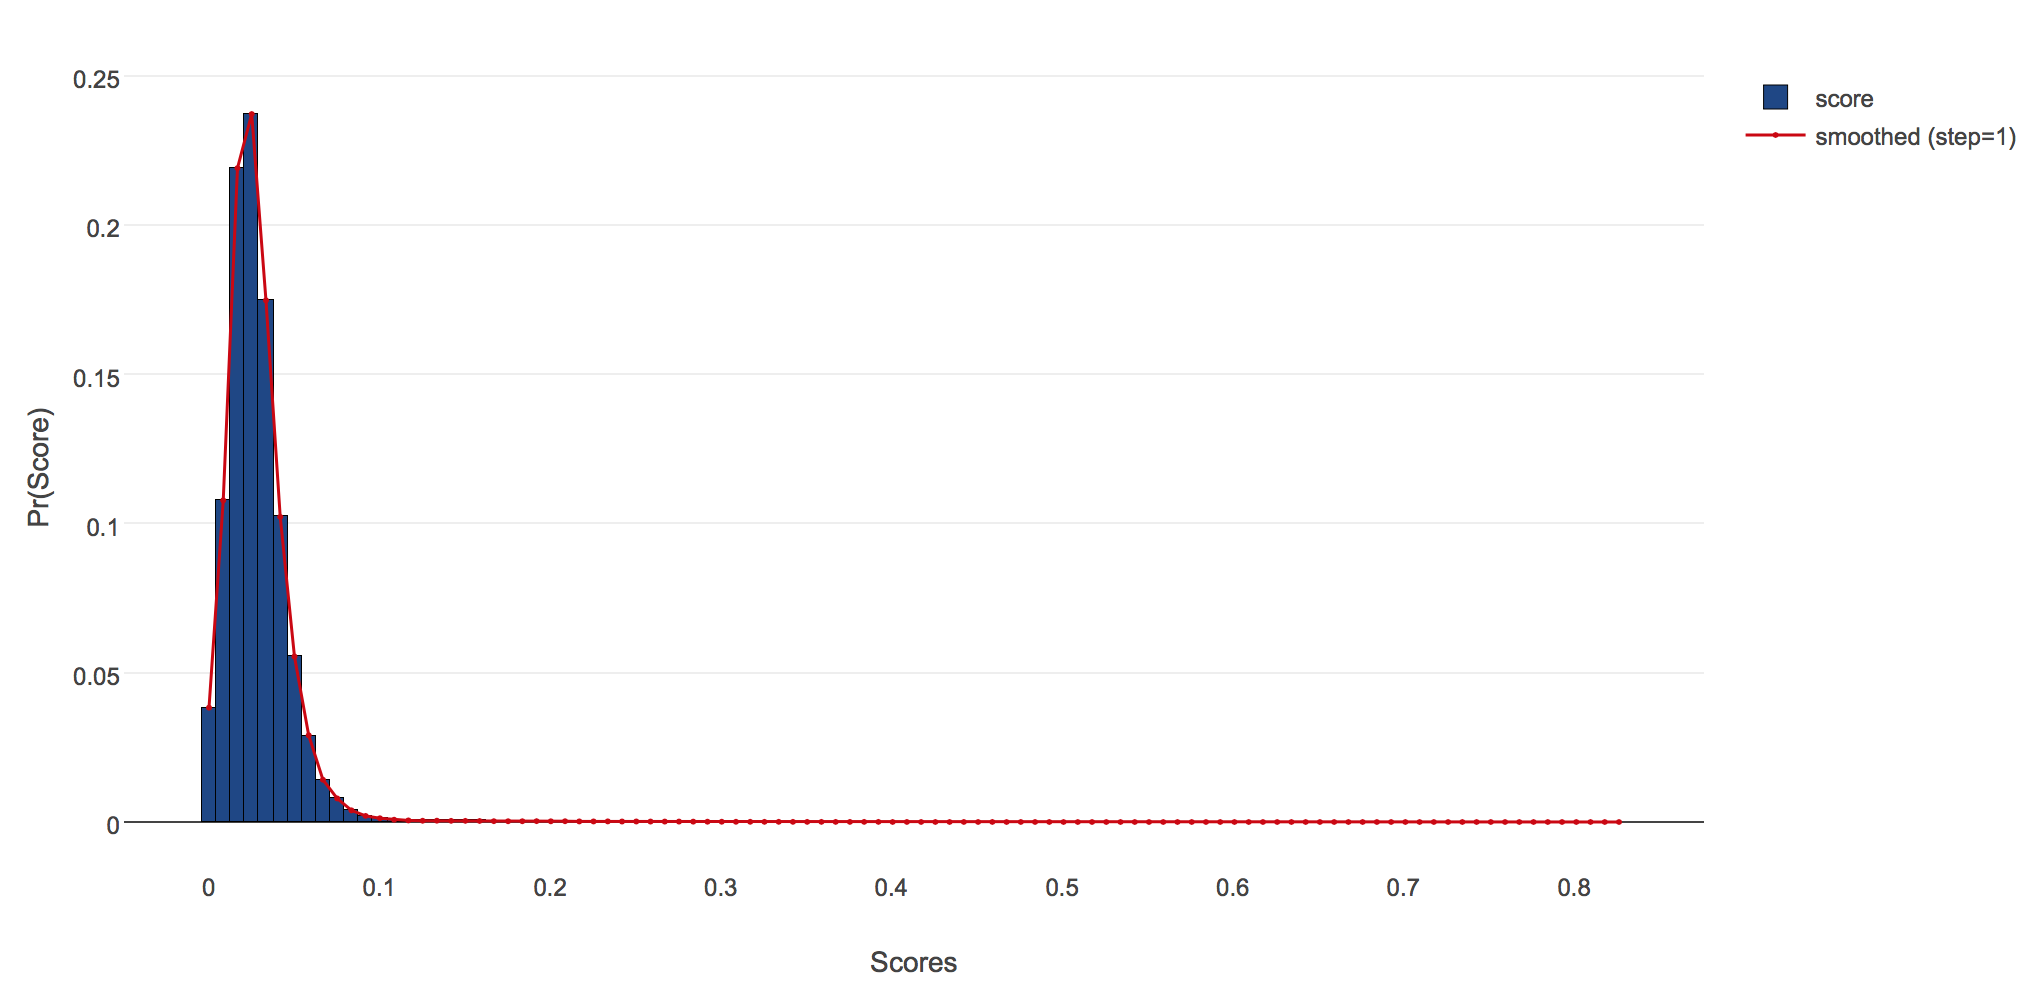
\includegraphics[height=2.7in]{dataset/grand/scores}
  \caption{Grand Score Distribution}
  \label{fig:grand_scores} %chktex 24
\end{subfigure}

 \begin{subfigure}[t]{\textwidth}
  \centering
  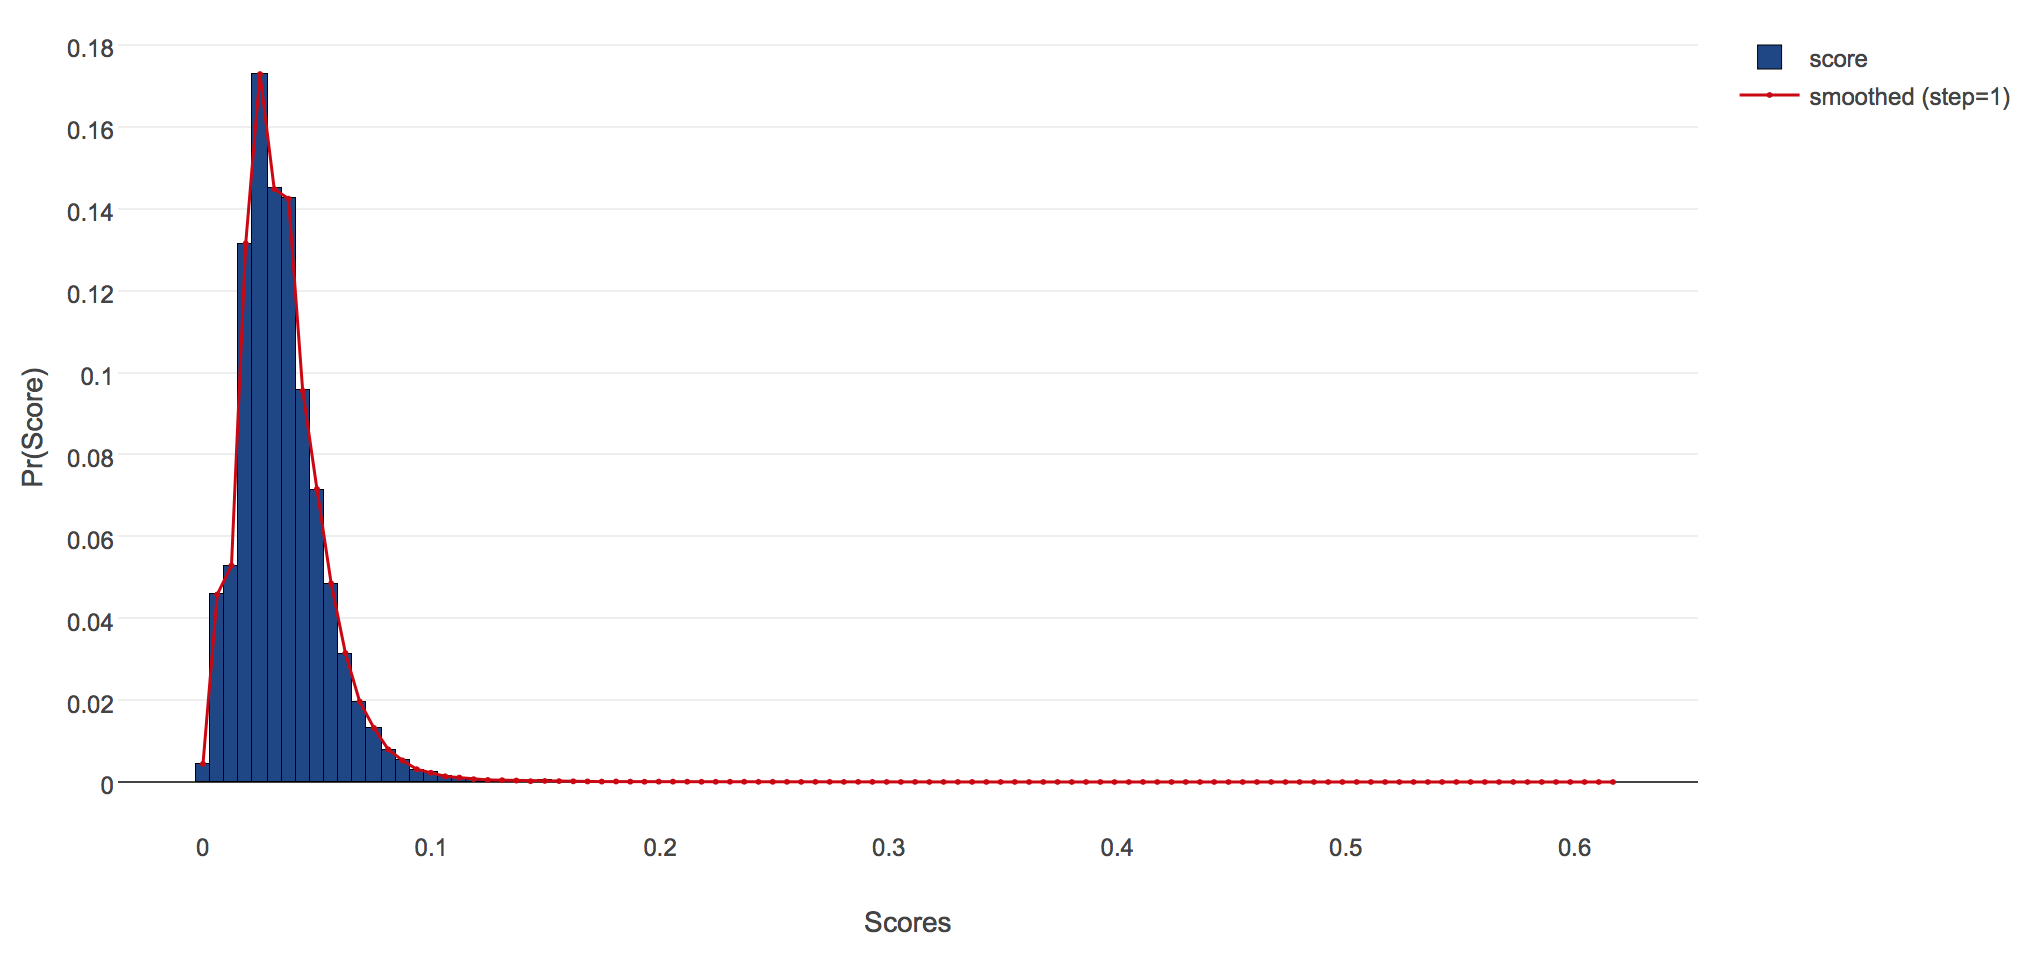
\includegraphics[height=2.5in]{dataset/otago/scores}
  \caption{Otago Score Distribution}
  \label{fig:otago_scores} %chktex 24
  \end{subfigure}
\end{figure}
